\chapter{Mulighetsanalyse}
\section{Beskrivelse av produkt/tjenestekonsept}
\subsection{Hvilket problem løses}
Kaffe er en viktig del av manges hverdag. Den har en oppkvikkende effekt og for mange er kaffekoppen fast inventar ved kontorplassen. Kaffen smaker best i et bestemt temperaturintervall (FINN UT: Høyst sannsynlig 60 - 80 grader \cite{bestekaffe} ), og det er et problem at kaffen er i dette temperaturintervallet i bare en kort tidsperiode. Det er et kjent problem at kaffen først er for varm og når man kjenner på den igjen er den for kald. Dermed faller kaffens smak betraktelig og mange ender med å skylle ut. Den ønskelige situasjonen er at kaffen holder seg i et konstant temperaturintervall. 

\subsection{Beskrivelse av produkt- og tjenestekonsept}
Vi tenker oss en kopp som på “magisk vis” holder innholdet på en behagelig, drikkbar temperatur. Dette realiseres gjennom en temperaturmåler og tilhørende mikrokontroller som befinner seg inne i koppen. Mikrokontrolleren drives av et lite batteri som lades ved hjelp av induksjon. I bunnen av koppen ligger et induksjonselement, som er atskilt væsken i koppen med en tynn plast-/glassfilm, for høy varmeledningsevne.

Koppen er avhengig av en induksjonsplate som den skal plasseres oppå, ikke ulikt dagens induksjonsladere for mobiltelefoner. På platen er det mulig å stille inn ønsket temperatur på drikken fra et lite temperaturintervall. I tillegg er det en lampe som lyser når drikken er under oppvarming. Både platen og koppen har RF-teknologi for å kommunisere med hverandre.

Når koppen settes ned på platen registrerer en trykksensor at koppen er satt ned, og maskineriet starter. Mikrokontrolleren slår seg på og leser av temperaturen på væsken i koppen. Informasjonen sendes direkte til induksjonsplaten, som prosesserer denne og starter med å varme innholdet til oppgitt temperatur. Deretter skapes det en konstant magnetisk fluks i platen slik at induksjonselementet blir varmt, og dermed varmer væsken i koppen. Denne fulksen lader også opp batteriet til mikrokontrolleren i koppen. 
Koppen sender relativt hurtige temperaturavlesninger til platen, og når det registreres temperaturer over grenseverdien, slutter platen å virke. Denne prosessen holder på så lenge koppen er plassert på platen. Hovedformålet er at innholdet i koppen skal kunne holde en konstant temperatur.

\subsection{Teknologiske utfordringer knyttet til produksjon og lansering}
Koppen skal inneholde en mikrokontrollerbrikke som skal kunne lese inn temperatur og opprettholde énveiskommunikasjon med induksjonsplaten. Et potensielt problem som kan oppstå er at brikken påvirkes av den høye temperaturen fra oppvarmingen av kaffen. Teknologien skal implementers i selve koppen, og må av den grunn kunne fungere optimalt selv når materialet rundt nærmer seg 100 grader. Mikrokontrolleren må også isoleres så koppen kan kjøres i oppvaskmaskinen uten at den blir skadet.

En annen utfordring ved produktet vårt ligger i det å få plass til all teknologien i to komponenter - kopp og plate - som i teorien skal være små i omfang. Koppen skal inneholde en liten metallplate av neglisjerbar størrelse, men mikrokontrolleren må få plass inne i selve materialet på koppen. Den skal også isoleres til en viss grad mot degraderende faktorer. Platen skal huse induksjonsledning, trykksensor og mikrokontroller - eventuelt annen teknologi for blant annet strøm - og som resultat av dette vil kunne bli større enn antatt. 

Av dette oppstår spørsmålet om produktet vårt vil få plass til all teknologien som skal til, og om koppen og platen må dimensjoneres større enn planlagt. Og om alle disse problemene løses, vil produktet med de funksjonene og den oppbygningen vi har bestemt oss for være lønnsomme å produsere?

Når det gjelder lanseringen ser vi ikke for oss at omfattende utfordringer vil oppstå, men det gjelder å være forberedt på at noen av produktene bærer feilproduksjon. Mikrokontrollerne er sensitive komponenter, og på grunn av påkjenninger (spesielt fra den varme væsken) vil noen kunder oppleve at produktet deres skades eller ødelegges innen garantitiden.

\section{Markedsbeskrivelse}
\subsection{Hvordan kan markedet overordnet segmenteres/inndeles?}
Vi ser for oss at dette produktet appelerer i høyest grad til personer som er glad i kaffe/te og som for det meste sitter på en fast plass og jobber, slik som i et kontor eller på en pult. Vi segmenterer markedet vårt demografisk. De mest interessante markedssegmentene for oss vil være 

\begin{itemize}
	\item Studenter
	\item Sittestillende arbeidsplasser(kontor, fast arbeidsplass)
	\item Alder
	\item Kjønn
\end{itemize}
Se markedsbeskrivelsen fra den andre gruppen på dette punktet. Her er det MYE bra.
\subsection{Kort om inngangsbarrierer}
- Vi er ukjente
- Forvirring rundt produktet (er dette en termokopp?)
- Produksjon
- Lite markedsføringsmidler
- Overbevise butikker om at det er et produkt verdt å selge
- Krever en del ressurser for å utvikle produktet
\paragraph{Markedsføring}
Det er mange store, etablerte produsenter som selger Termokopper, f.eks. Bodum \cite{bodum}. Disse her et mye høyere markedsføringsbudsjett enn oss, og kommer høyst sannsynlig til å være synligere i butikkhyllene enn oss. Det å nå ut til folket og gjøre potensielle kunder oppmerksomme på produktet kommer til å bli en utfordring.

Det er også et produkt folk ikke har sett så mye til før. Vi kan derfor se for oss at det kan bli et problem at kundene ikke ser forskjell på HeatPledger og en mer normal kopp eller termokopp ved første øyekast. Dette må være i bakhodet når embalasjen skal designes.

\paragraph{Utvikling og produksjon av HeatPledger}
Utviklingen av HeatPledger kommer til å kreve teknologisk innsikt, samtidig som det kommer til å brukes en del tid på å designe produktet. På laget er vi 5 dataingeniører, så den teknologiske biten burde muliggens gå bra, men det er mulig vi kan trenge vi kan trenge en produktdesigner. Dette er dyrt, og kan bli en stor utgiftspost.

\paragraph{Avtaler}
For å komme inn i et etabler marked er det en fordel å ha avtale med store aktører som finnes i markedet, da spesielt med tanker på distributører. Det vil være naturlig å ta kontakt med elektronikkbutikker som Lefdal, Expert og Elkjøp, i tillegg til rene nettbutikker som komplett.no. HeatPledger passer også inn i butikker slik som Enklere Liv og Teknikkmagasinet, som selger forskjellige produkter som skal gjøre hverdagen litt enklere. Og sist men ikke minst vil det være naturlig å etablere et samarbeid med kjeder som Kitchn, Tilbords og andre butikker som selger kjøkkenartikler. Det vil være viktig for oss at distributørene kan overbevises om at dette er et produkt de ønsker å selge videre. Gjennom kommunikasjonen vi har hatt med de forskjellige kjedene (se kapittel 3), virker det som om det er flere distributører som synes ideen virker atraktiv.

\paragraph{Startkapital}
Det kommer til å være nødvendig med en startkapital stor nok til å kunne utvikle produktet og få produsert de første enhetene av HeatPledger. Kostnadene kommer til å avhenge av mange faktorer som produksjonskostnader og hvor mye ekstern kompetanse vi kommer til å trenge å leie inn for å få fullført produktet. 

\subsection{Kort om konkurrenter og substitutter}
Innen kaffemarkedet finnes det mange forskjellige produkter som dekker mange forskjellige behov. Termokoppen som er et veldig vanlig produkt i dagens marked, kan fungere som et substitutt for vårt produkt. Som en representant for Expert svarer oss på mail i spørsmål om produktet vårt er av interesse for dem og om de tror det er marked for det: "Produktet i seg selv er innovativt og kan være en mulighet, men utfordringen er nok at en god thermos kopp / eller to-go kopp gjør samme nytten og holder på varmen i flere timer uten at en tilkobling til strøm er nødvendig." Av direkte konkurrenter er det veldig lite ute på markedet akkurat nå. Teknikkmagasinet skriver i en mail til oss at de har et produkt med omtrent samme funksjonalitet, men at det fungerer på en litt annen måte enn vårt produkt gjør. Produktet vårt er likevel mer avansert, av bedre kvalitet og konkurrerer derfor om to forskjellige kundegrupper. Produktet Teknikkmagasinet linker til \cite{tmprod} klarer for eksempel ikke å gi nok effekt til å holde kaffen i optimal drikketemperatur (60 grader Celcius \cite{optimaldrikketemperatur}).

Av andre aktører som selger produkter i vår produktkategori var det også en representant fra butikkjeden Tilbords som uttalte seg om vårt produkts relevans i dagens marked: "Hvis det kun er en noe som skal holde kaffen varm tror jeg dette blir et marginalt produkt. En kopp kaffe drikker du så fort at du ikke trenger å holde den varm." Det kan derfor se ut til at representanter fra Tilbords er tvilende til om produktet har noe salgspotensial. Teknikkmagasinet er mer optimistiske og skriver i mailen til oss at det absolutt er et produkt de kunne tenke seg å selge. Representanten fra Expert uttaler også meninger som peker i samme retning: "Spennende med nye produkter innenfor kaffe, spesielt siden Norden drikker mest kaffe pr person i verden. (...) Det som taler for produktet er at det finnes mye gadgets man kan kjøpe til kontorpulten sin, alt fra USB vifter til rare duppedingser som kobles til strøm og har en eller annen funksjon på pulten."

Representanter fra bransjen ser derfor ut til å ha delte meninger, og det er derfor spennende å se nærmere på resultatene fra markedsundersøkelsen vår som et supplement til deres antagelser.

Her kommer det frem at drøye 50\% av dem som drikker kaffe eller andre varme drikker, sier at de hadde vært interessert i et slikt produkt som vi beskriver om det hadde eksistert i dag. I tillegg svarer ca. 32\% av disse igjen at de kanskje hadde vært interessert.



\section{Om organisering og økonomisk potensial}
\subsection{Forretningsmodell}
Vi ønsker å selge HeatPledger direkte til akutelle distributører, altså butikker som Expert, Enklere Liv og Tilbords, i tillegg til nettbutikker som komplett.no. Distributørene vil kontaktes direkte, og varene vil fraktes dit med allerede eksisterende transportselskaper slik som Posten eller DHL. På denne måten vil produktene kunne spres til mange butikker på kort tid, noe som kan være fordelaktig for salget.

En ulempe med å selge produktet gjennom en distributør på denne måten er at vi får et ekstra fordyrende mellomledd, som kan føre til at produktet kan bli dyrere til sluttbruker og/eller gi oss mindre profitt. 

En annen ulempe med denne løsningen er at vi i mindre grad styrer eksponeringen av produktet og ikke retter seg like godt ut mot sluttbruker som antat. Dette er dog risikoer vi må leve med og vi mener fordelene ved å gå for denne løsningen overgår ulempene.
\subsection{Organisering}



\subsection{Hva gjør vi selv, hva outsourcer vi?}



\subsection{Økonomisk potensial}
Som det er sett på tidligere i rapporten, er det mange mennesker som er i målgruppen for dette produktet. Det er derfor muligheter for å selge mange enheter av produktet om det markedsføres riktig og slår bra an.

Utifra spørreundersøkelsen vi har holdt, kan vi lese at andelen at det er en gjevn fordeling mellom de som synes det viktigste med produktet er at det er billig og de som synes det viktigste er kvalitet. Det er derfor muligheter for å selge flere versjoner av koppen. En enklere billigversjon og en litt dyrere "premiumutgave". Her er det mulighet for å hente ut ekstra profitt på premiumversjonen.

Som vi har sett på tidligere, er det vanskelig for oss å oppnå en utsalgspris på mindre enn 300 kr. 
Samtidig kan vi lese av undersøkelsen at hele 93\% av de som svarte maksimalt ville ha betalt \textit{under} 300 kr for koppen. Dermed kan det tyde på at produktet vårt kan bli for dyrt til at det virkelig kan slå an i de store massene.

\begin{figure}
\centering
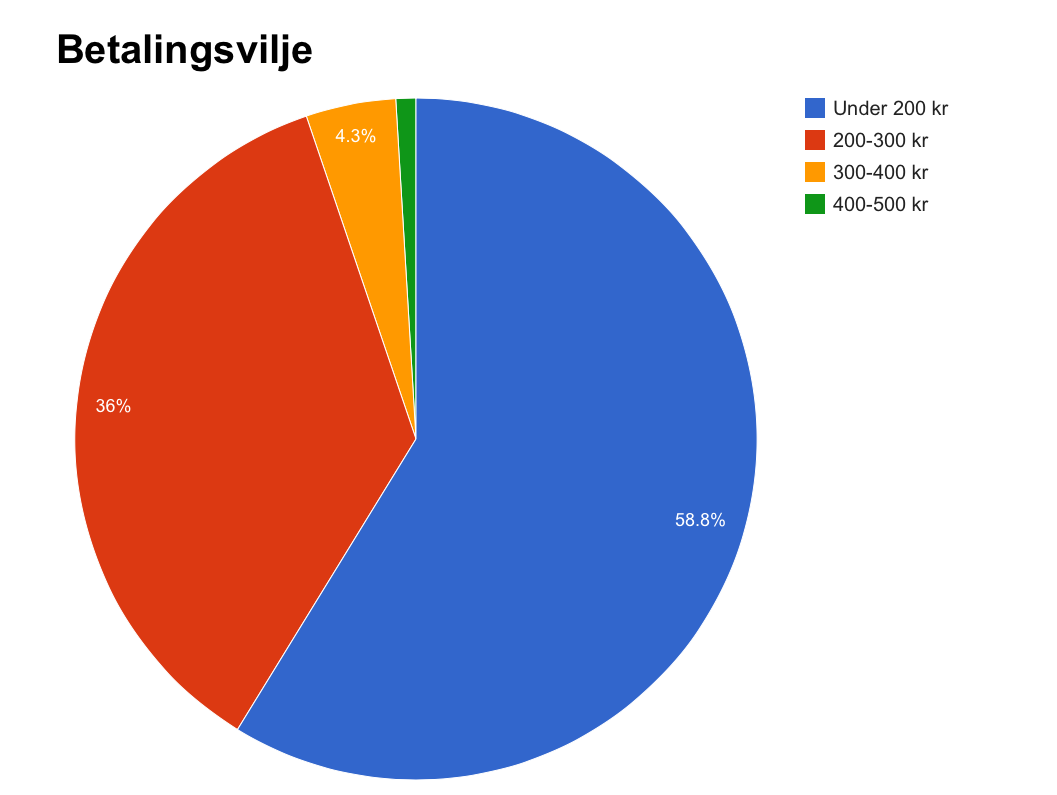
\includegraphics[scale=0.3]{images/ModelForBetalingsvilje.png}
{\caption{\textit{\scriptsize Svar på spørsmålet: Hvor mye er du maksimalt villig til å betale for et slikt produkt?}}}
\label{fig:betalingsvilje}
\end{figure} 

Pass på å nevne noe her om hvor mange enheter vi må selge for å gå i pluss. 
Hent svar fra spørreundersøkelse (hvor mye er folk villig til å betale for koppen vår kontra hvor mye kommer det kommer til å koste å produsere den? Se andre rapporten for inspirasjon.)

\subsection{Finansieringsbehov og finansieringskilder}
Hvor mye kommer koppen til å koste? Hvor mye kreves i startkapital? Hvordan skal vi få tak i pengene? Se diskusjon ang startkapital i seksjon 2.2.2.
Hvor har vi tenkt å få den evt startkapitalen fra? Se rapport fra annen gruppe. Her står det mye spennende.
